\chapter{Implementación en Fabric}
\section{Diseño}
\subsection{Registro}
Debido a que en Fabric se utiliza una base de datos (\textit{world state}) para almacenar datos, no es necesario crear estructuras de datos en memoria para guardar las credenciales y las presentaciones. Ambas se crean en formato clave-valor, utilizando su \acrshort{psmhash} como clave y un objeto JSON con toda la información relevante como valor. Solo se utiliza un objeto credencial, y se diferencia entre credenciales de emisor o de sujeto mediante un campo ``type'' en el JSON de cada credencial.

\begin{figure}[H]
\centerline{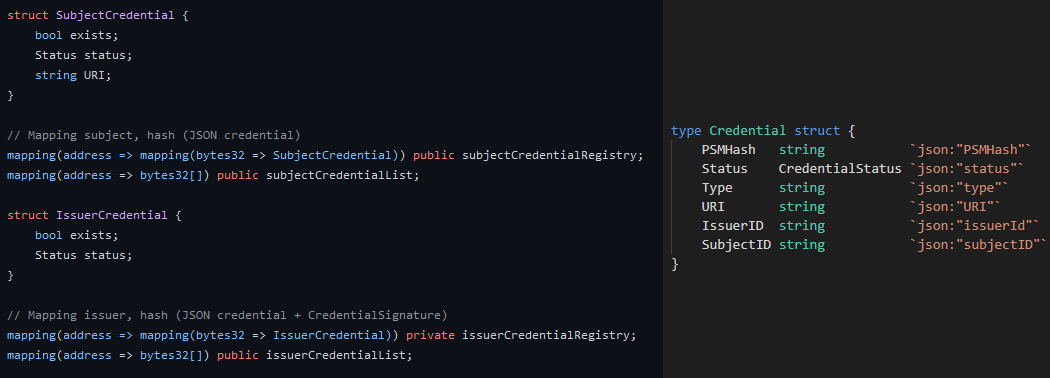
\includegraphics[scale=0.55]{recursos/subjectcredential.png}}
\caption{Comparación Credential entre Solidity y Go.}
\label{credential-comp}
\end{figure}
En la imagen a la izquierda está la implementación en Solidity y a la derecha en Go, se puede observar que en Go solo se utiliza un objeto para todo tipo de credenciales, y que no se utilizan mappings para almacenarlas, ya que en Fabric los datos se guardan en el \textit{world state}. Los campos específicos de las credenciales de sujeto se quedaran vacíos en las de emisor, y viceversa.

\begin{figure}[H]
\centerline{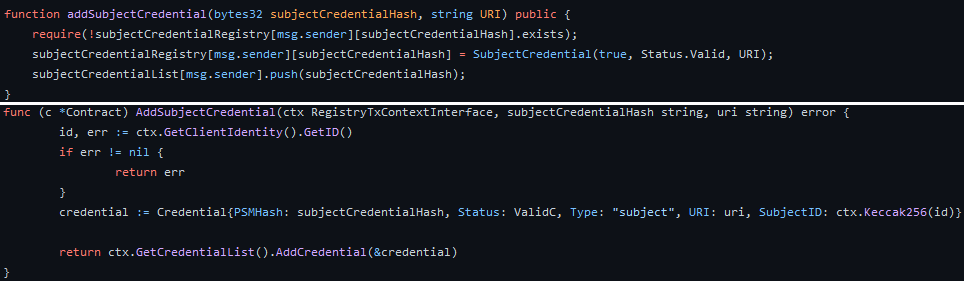
\includegraphics[scale=0.60]{recursos/addsubjectcredential.png}}
\caption{Comparación de la función addSubjectCredential entre Solidity y Go.}
\label{add-credential-comp}
\end{figure}
En la imagen arriba está la implementación en Solidity y abajo en Go de la función ``AddSubjectCredential'', para añadir credenciales de sujeto. Como se puede observar, en Go se crea un objeto JSON con los datos y se guarda en el \textit{world state}, rellenando en este caso el campo SubjectID con el ClientID del llamante hasheado con keccak256. Se ha optado por esta función de hash para que sea lo mas similar posible a la implementación Solidity, pero se podrían utilizar otros algoritmos. La función ``AddIssuerCredential'', que sirve para añadir credenciales de emisor, sería identica, salvo por que en el objeto credencial se rellenaría el campo IssuerID y se dejaría el campo URI vacío.

En el caso de las presentaciones el funcionamiento es prácticamente idéntico, con un solo objeto presentación y un campo ``type'' para diferenciar entre sujeto y receptor.
\subsection{Identidad}
En lo referente a entidades, se eliminan los objetos de emisor y proveedor de servicios, y se concentran en un objeto Entity, que se define como uno u otro mediante atributos booleanos ``isIssuer'' e ``isServiceProvider''. Esto además soluciona el problema de que una entidad pudiera tener un rol sin ser técnicamente ``entity''.
\begin{figure}[H]
\centerline{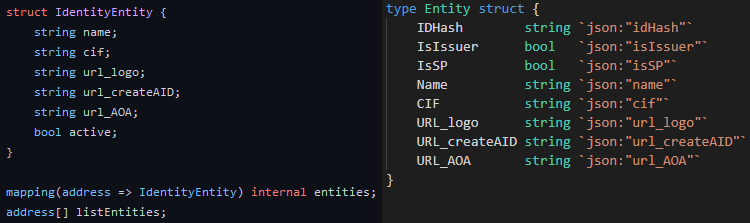
\includegraphics[scale=0.8]{recursos/entities.png}}
\caption{Comparación Entity entre Solidity y Go.}
\label{entities-comp}
\end{figure}
En la imagen a la izquierda esta la implementación en Solidity y a la derecha en Go del objeto Entity. En la implementación en Solidity, este objeto solo contiene la información sobre la entidad, pero para almacenar entidades emisoras o proveedoras de servicio utiliza otras estructuras, repartidas en dos smart contracts. En Go, se elimina la necesidad de estos dos smart contracts y se concentran las entidades en un solo objeto, que tiene los mismos campos que en Solidity más tres campos extra que indican el rol de la entidad y la identidad que le corresponde. Una vez más, no es necesario el mapping en Go ya que los datos se almacenan en el \textit{world state}.

En Quorum, cada entidad está representada por una dirección propia y fácilmente manejable. En Fabric, cada entidad representaría a una organización, pero como las organizaciones no tienen un certificado propio ni nada que las identifique como tal, se utilizaría una identidad estándar para representar a cada entidad/organización, y cada una de ellas accedería a la blockchain como si fuera un sujeto, a través de un wallet de identidad. Dentro de los chaincodes es donde se reconocería a cada identidad como entidad o sujeto. 

En la implementación de Solidity existe un problema con los nuevos despliegues, y es que se necesita una primera entidad emisora para poder empezar a crear identidades. La antigua solución era crear la primera entidad a mano utilizando la cuenta de administrador, pero con los nuevos smart contracts en desarrollo, el problema se soluciona mediante un parámetro pasado en la inicialización de los contratos. En Fabric surge el mismo problema, pero se puede aplicar la misma solución que en Solidity, creando esa primera entidad en la inicialización del chaincode.

Todo el funcionamiento de la entidad, ya sea emisora, proveedora de servicios, o ninguna de los dos, se ha concentrado en un solo smart contract, que realizará todas las gestiones pertinentes.

En cuanto a la creación de identidades, se eliminan los AlastriaProxy, pero el resto del funcionamiento se mantiene similar. Las identidades se almacenan como un objeto JSON con tres atributos.
\begin{figure}[H]
\centerline{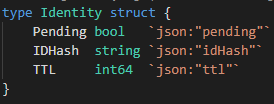
\includegraphics[scale=1]{recursos/identity.png}}
\caption{Objeto JSON que representa las identidades.}
\label{identity-json}
\end{figure}
\begin{itemize}
    \item \textbf{Pending:} Booleano que se activa cuando un emisor inicia el proceso de creación de la identidad. Es el equivalente a la función ``prepareAlastriaID'' en los contratos en Solidity.
    \item \textbf{IDHash:} String que representa el identificador de la identidad. En la implementación en Solidity se utiliza la dirección del AlastriaProxy correspondiente, pero como en este modelo no existen los proxies, se utiliza un hash keccak256 del ClientID del sujeto al que se le va a crear la identidad.
    \item \textbf{TTL:} Time To Live. Tiempo en formato UNIX que no se debe haber superado a la hora de crear la identidad.
\end{itemize}
Debido a que no es posible el uso de proxies, la creación de AlastriaIDs quedaría limitada a uno por ClientID, a diferencia de la implementación en Solidity. Puesto que no se puede crear mas de una identidad por sujeto, no se puede implementar la función de recuperación de cuentas.

Respecto a la creación de identidades y los IDHashes, una alternativa sería que la propia organización ya almacenase los ClientID en formato hash, así no haría falta hashearlos en el propio chaincode.

\section{Implementación}
La implementación de los smart contracts para la red Fabric está hecha en Go, y la base de datos que se utiliza para el world state es LevelDB, para cuyas búsquedas se crean claves compuestas con la información relevante. Otra opción sería usar CouchDB, que permite la búsqueda por valor y no solo por clave, lo que facilita mucho las búsquedas, aunque requiere cambiar configuración de la red y preestablecer unos índices que, de crecer mucho, podrían afectar al rendimiento de la red. Todos los hashes utilizan la función Keccak256, para mantener el paralelismo con la implementación en Solidity, aunque se podrían usar otras funciones de hash si así se quisiese.\\

La red utilizada es la red de pruebas facilitada en el GitHub oficial de Fabric, con utilidades para desplegar rápidamente una red con dos organizaciones y todos los nodos necesarios para desplegar chaincodes inmediatamente. Los nodos se despliegan mediante contenedores Docker, así como los chaincodes. Aun así, los chaincodes podrían desplegarse en cualquier red Fabric.
\begin{figure}[H]
\centerline{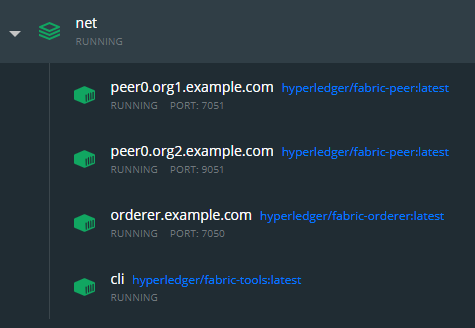
\includegraphics[scale=0.9]{recursos/network-daocker.png}}
\caption{Contenedores Docker con los nodos de la red.}
\label{docker-net}
\end{figure}
En la imagen se puede observar la red Docker de pruebas, con un \textit{peer} por organización y un \textit{orderer} común. El contenedor CLI es la consola de Fabric. Los chaincodes se despliegan en contenedores independientes.

\begin{figure}[H]
\centerline{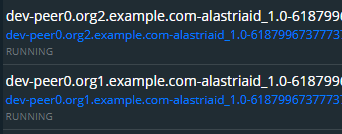
\includegraphics[scale=0.9]{recursos/chaincodes-docker.png}}
\caption{Contenedores Docker con los chaincodes.}
\label{chaincodes-docker}
\end{figure}
En la imagen se pueden observar dos contenedores, pero contienen el mismo chaincode, porque cada organización lo despliega independientemente después de llegar a un acuerdo.

Las identidades se han generado utilizando la herramienta Cryptogen, diseñada solo para entornos de pruebas. En una red real las identidades son gestionadas por las autoridades de certificación (CA), organizaciones que emiten certificados e identidades digitales. 

Por falta de tiempo, solo se ha realizado la implementación del grupo \textbf{API Ledger}, de \textbf{identityManager.go}, y de los contratos de gestión de credenciales.